%&preformat-synopsis
\RequirePackage[l2tabu,orthodox]{nag} % Раскомментировав, можно в логе получать рекомендации относительно правильного использования пакетов и предупреждения об устаревших и нерекомендуемых пакетах
\PassOptionsToPackage{bookmarks=false}{hyperref}
%\documentclass[a5paper,10pt,twoside,openany,article]{memoir} %,draft
\documentclass[a4paper,14pt,oneside,openany]{memoir}

\input{common/setup}        % общие настройки шаблона
\input{common/packages}     % Пакеты общие для диссертации и автореферата
\synopsistrue               % Этот документ --- автореферат
\input{Report/reppackages}  % Пакеты для автореферата
\usepackage{amsmath} {
	\theoremstyle{plain}
	\newtheorem{assumption}{Предположение}
} % Пакеты для специфических пользовательских задач
\usepackage{amsmath} {
	\theoremstyle{plain}
	\newtheorem{assumption}{Предположение}
}

\input{common/newnames}     % Новые переменные, которые могут использоваться во всём проекте
\input{Report/setup}        % Упрощённые настройки шаблона

\input{common/data}         % Основные сведения
\input{common/fonts}        % Определение шрифтов (частичное)
\input{common/styles}       % Стили общие для диссертации и автореферата
%\input{Report/disstyles}   % Стили для диссертации
%%% Изображения %%%
\graphicspath{{images/}{Synopsis/images/}}         % Пути к изображениям

%%% Макет страницы %%%
\geometry{a4paper, top=2cm, bottom=2cm, left=2.5cm, right=1cm, nofoot, nomarginpar} %, heightrounded, showframe
\setlength{\topskip}{0pt}   %размер дополнительного верхнего поля

%%% Интервалы %%%
%% Реализация средствами класса (на основе setspace) ближе к типографской классике.
%% И правит сразу и в таблицах (если со звёздочкой)
%\DoubleSpacing*     % Двойной интервал
\OnehalfSpacing*    % Полуторный интервал
%\SingleSpacing      % Одинарный интервал
%\setSpacing{1.42}   % Полуторный интервал, подобный Ворду (возможно, стоит включать вместе с предыдущей строкой)

%%% Выравнивание и переносы %%%
%% http://tex.stackexchange.com/questions/241343/what-is-the-meaning-of-fussy-sloppy-emergencystretch-tolerance-hbadness
%% http://www.latex-community.org/forum/viewtopic.php?p=70342#p70342
\tolerance 1414
\hbadness 1414
\emergencystretch 1.5em % В случае проблем регулировать в первую очередь
\hfuzz 0.3pt
\vfuzz \hfuzz
%\raggedbottom
%\sloppy                 % Избавляемся от переполнений
\clubpenalty=10000      % Запрещаем разрыв страницы после первой строки абзаца
\widowpenalty=10000     % Запрещаем разрыв страницы после последней строки абзаца

%%% Колонтитулы %%%
\makeevenhead{plain}{}{}{}
\makeoddhead{plain}{}{}{}
\makeevenfoot{plain}{}{\thepage}{}
\makeoddfoot{plain}{}{\thepage}{}
\pagestyle{plain}

%%% Размеры заголовков %%%
\setsecheadstyle{\normalfont\large\bfseries}
\renewcommand*{\chaptitlefont}{\normalfont\large\bfseries}

%%% Подписи %%%
\setfloatadjustment{table}{%
    \setlength{\abovecaptionskip}{0pt}   % Отбивка над подписью
    \setlength{\belowcaptionskip}{0pt}   % Отбивка под подписью
}

%%% Отступы у плавающих блоков %%%
\setlength\textfloatsep{1ex}

\renewcommand{\cftchapterdotsep}{\cftdotsep}                % отбивка точками до номера страницы начала главы/раздела

\makechapterstyle{thesisgost}{%
	\chapterstyle{default}
	\setlength{\beforechapskip}{0pt}
	\setlength{\midchapskip}{0pt}
	\setlength{\afterchapskip}{\theintvl\curtextsize}
	\renewcommand*{\chapnamefont}{\basegostsectionfont}
	\renewcommand*{\chapnumfont}{\basegostsectionfont}
	\renewcommand*{\chaptitlefont}{\basegostsectionfont}
	\renewcommand*{\chapterheadstart}{}
	\ifnumgreater{\value{headingdelim}}{0}{%
		\renewcommand*{\afterchapternum}{.\space}   % добавляет точку с пробелом после номера раздела
	}{%
		\renewcommand*{\afterchapternum}{\quad}     % добавляет \quad после номера раздела
	}
	\renewcommand*{\printchapternum}{\hdngaligni\hdngalign\chapnumfont \thechapter}
	\renewcommand*{\printchaptername}{}
	\renewcommand*{\printchapternonum}{\hdngaligni\hdngalign}
}


    % Стили для автореферата
\newcommand\blank[1][\textwidth]{\noindent\rule[-.2ex]{#1}{.4pt}}

\usepackage{titlesec}
\titleformat{\chapter}[hang] 
{\normalfont\large\bfseries}{\thechapter.}{1em}{}    % Стили для специфических пользовательских задач
%%% Мои макросы
\newcommand{\bm}[1]{\boldsymbol{#1}}
\newcommand{\ten}[1]{\bm{\mathcal #1}} % tensor
\newcommand{\set}[1]{{\mathcal #1}}    % set
\newcommand{\compl}{\mathbb{C}}        % complex-valued numbers
\newcommand{\real}{\mathbb{R}}         % real-valued numbers
\newcommand{\eqdef}{\stackrel{.}{=}} % definition
\DeclarePairedDelimiter{\ceil}{\lceil}{\rceil}
\DeclarePairedDelimiter{\floor}{\lfloor}{\rfloor}
\newcommand{\te}[1]{\mathrm{#1}}
\newcommand{\at}[2][]{#1|_{#2}}

%% Часто используемые символы
\newcommand{\ta}{t}
\newcommand{\ti}{k}
\newcommand{\Nt}{N_t}
\newcommand{\ts}{T}
\newcommand{\fri}{i}
\newcommand{\Nf}{N_f}
\newcommand{\fra}{f}
\newcommand{\scs}{\Delta_f}
\newcommand{\spi}{j}
\newcommand{\Ns}{N_j}
\newcommand{\rxi}{{m}}
\newcommand{\Nrx}{{M}}
\newcommand{\txi}{{n}}
\newcommand{\Ntx}{{N}}
\newcommand{\spa}{\bm{p}}
\newcommand{\pars}{{\bm{\Theta}}}
\newcommand{\Npars}{{P}}
\newcommand{\pai}{{l_\txi}}
\newcommand{\Npa}{{L_{\txi}}}
\newcommand{\hpa}{{h_\pai}}
\newcommand{\Spai}{{\set{L}_\txi}}
\newcommand{\tgain}{{\tilde{\alpha}}}
\newcommand{\tgaini}{{\tgain_{\pai}}}
\newcommand{\gain}{{\alpha}}
\newcommand{\gaini}{{\gain_{\pai}^{\ti}}}
\newcommand{\lfr}{f_\te{L}}                              % lowest frequency
\newcommand{\ufr}{f_\te{U}}                              % up'est frequency
\newcommand{\cfr}{f_\te{C}}                              % center (carrier) frequency
\newcommand{\sfr}{f_\fri}                                % carrier frequency
\newcommand{\fulldelay}{\tilde{\tau}_{\pai}^{\txi,\rxi}} % full time delay
\newcommand{\delay}{\tau_{\pai}}                         % delay
\newcommand{\vrel}{v_{\pai}}                             % relative velocity
\newcommand{\deltx}{{\delta_{\txi,\pai}^\te{t}}}         % transmit antenna geometric path difference
\newcommand{\delrx}{{\delta_{\rxi,\pai}^\te{r}}}         % receive antenna geometric path difference
\newcommand{\di}{{d_\pai}}                               % distance between reference transmit and receive antennas






%%% Библиография. Выбор движка для реализации %%%
\ifnumequal{\value{bibliosel}}{0}{%
    \input{biblio/predefined} % Встроенная реализация с загрузкой файла через движок bibtex8
}{
    \input{biblio/biblatex}   % Реализация пакетом biblatex через движок biber
}

% Вывести информацию о выбранных опциях в лог сборки
\typeout{Selected options:}
\typeout{Draft mode: \arabic{draft}}
\typeout{Font: \arabic{fontfamily}}
\typeout{AltFont: \arabic{usealtfont}}
\typeout{Bibliography backend: \arabic{bibliosel}}
\typeout{Precompile images: \arabic{imgprecompile}}
% Вывести информацию о версиях используемых библиотек в лог сборки
\listfiles

\begin{document}

\thispagestyle{empty}


%\large
\begin{center}
\textbf{ 
федеральное государственное бюджетное образовательное учреждение\\ высшего образования\\
<<Казанский национальный исследовательский университет\\им. А.Н. Туполева-КАИ>>}
\end{center}

\vspace{0pt plus1fill} %число перед fill = кратность относительно некоторого расстояния fill, кусками которого заполнены пустые места


\vspace{0pt plus3fill} %число перед fill = кратность относительно некоторого расстояния fill, кусками которого заполнены пустые места

\begin{center}
	\textbf {Научный доклад об основных результатах подготовленной научно-квалификационной работы на тему: \\%\MakeUppercase
<<\thesisTitle>>}
\end{center}


\vspace{0pt plus3fill} %число перед fill = кратность относительно некоторого расстояния fill, кусками которого заполнены пустые места

\hfill\begin{minipage}[h]{0.5\linewidth}
аспиранта очной формы \\
4 года подготовки\\
кафедры РТС \\
Подкуркова Ивана Алексеевича
\\\\
направление подготовки:\\ \thesisSpecialtyNumber\  <<\thesisSpecialtyTitle>>
\\\\
направленность (профиль):\\ \thesisSpecialtyTwoNumber\  <<\thesisSpecialtyTwoTitle>>
\\\\
отрасль науки: технические \\
научный руководитель: \\
д.ф.-м.н., профессор Надеев Адель Фирадович
\end{minipage}


%
%направление подготовки 
%11.06.01 «Электроника, радиотехника и системы связи»
%
%направленность (профиль)
%05.12.13 «Системы, сети и устройства телекоммуникации»
%



\vspace{0pt plus4fill} %число перед fill = кратность относительно некоторого расстояния fill, кусками которого заполнены пустые места
{\centering\thesisCity~ \thesisYear\par}

\newpage
        % Титульный лист
%\input{Report/contents}      % Таблица с Содержание автореферата
\tableofcontents*
\clearpage
%\mainmatter                   % В том числе начинает нумерацию страниц арабскими цифрами с единицы
%\mainmatter*                  % Нумерация страниц не изменится, но начнётся с новой страницы
\chapter{Общая характеристика работы}

\newcommand{\actuality}{\underline{\textbf{\actualityTXT}}}
\newcommand{\progress}{\underline{\textbf{\progressTXT}}}
\newcommand{\object}{\underline{{\textbf\objectTXT}}}
\newcommand{\predmet}{\underline{{\textbf\predmetTXT}}}
\newcommand{\aim}{\underline{{\textbf\aimTXT}}}
\newcommand{\tasks}{\underline{\textbf{\tasksTXT}}}
\newcommand{\novelty}{\underline{\textbf{\noveltyTXT}}}
\newcommand{\influence}{\underline{\textbf{\influenceTXT}}}
\newcommand{\methods}{\underline{\textbf{\methodsTXT}}}
\newcommand{\defpositions}{\underline{\textbf{\defpositionsTXT}}}
\newcommand{\reliability}{\underline{\textbf{\reliabilityTXT}}}
\newcommand{\probation}{\underline{\textbf{\probationTXT}}}
\newcommand{\contribution}{\underline{\textbf{\contributionTXT}}}
\newcommand{\publications}{\underline{\textbf{\publicationsTXT}}}
\newcommand{\passconf}{\underline{\textbf{\passconfTXT}}}


{\actuality} Развитие новых методов модуляции с множеством поднесущих и систем передачи данных с множеством входных и выходных портов (MIMO) увеличивают количество получаемой информации и приводят к тому, что сигналы в таких системах могут быть описаны как многомерные массивы данных - тензоры, представляющие собой дискретизацию многомерных непрерывных сигналов.

Тензорное представление сигналов и моделей каналов связи открывает новые возможности к оцениванию параметров таких сигналов с помощью тензорных разложений. Такие тензорные разложения обладают свойствами уникальности и идентифицируемости, которые необходимы для корректного извлечения полезной информации из принимаемых сигналов и, помимо этого, могут сами нести полезную информацию в определённых сценариях.

Вместе с тем, увеличение объёма получаемой информации приводит к увеличению требований к вычислительным ресурсам таких систем. Моделирование передаточных функций каналов связи как полностью случайных и неизвестных стохастических величин приводит к нереализуемым методам и алгоритмам. Поэтому, в данной работе рассматриваются параметрические модели каналов связи \cite{Richter2005}, позволяющие уменьшить количество свободных параметров каналов связи тем самым снизив требования к вычислительным ресурсам систем связи, а также увеличив эффективность их эквализации.

Новые инфокоммуникационные системы, в погоне за растущими потребностями в пропускной способности, постоянно наращивают используемые ресурсы, чаще всего за счёт использования большей полосы частот. Увеличение относительных полос частот этих систем приводит к несостоятельности традиционных моделей данных в них, и, как следствие, алгоритмов оценивания параметров \cite{DoHong2004, Raimondi2016}. В данной работе предлагается общая методика обработки получаемых данных, позволяющая применять узкополосные алгоритмы оценивания параметров каналов связи - направлений прихода сигналов на массив антенн - в широкополосных системах.

Сферическая модель фронта волны даёт возможность оценивать с помощью массива антенн не только направления прихода сигналов, но и расстояния до источника сигнала или его последнего отражения \cite{Singh2017a, Singh2017}. Получение с помощью тензорных разложений несмещенных оценок фазовых сигнатур приходящих на массив антенн сигналов позволяет применять новые методы определения местоположения источников сигналов и их отражателей в ближнем геометрическом поле \cite{Singh2016}. В данной работе предлагается новый алгоритм оценивания направлений прихода сигналов и расстояния до его источника в ближнем геометрическом поле.

Растущая насыщенность частотного спектра приводит к усложнению внутренних и внешних помех в современных инфокоммуникационных системах, что, в свою очередь, приводит к несостоятельности простых статистических моделей аддитивных помех в виде часто используемого белого шума с нормальным распределением \cite{Kozick2000, Kalyani2012}. Это оправдывает использование более сложных статистических моделей аддитивных помех в таких системах, например, таких как смесей нормальных распределений. Введение более сложных моделей аддитивных помех приводит к необходимости анализа потенциальных характеристик оценивания параметров сигналов, в качестве которых распространено использование нижней границы Крамера-Рао \cite{Cramer1993, KayS.1993}. В данной работе предлагается обобщенный метод расчёта потенциальных характеристик оценивания параметров каналов связи с учётом негауссовских распределений аддитивных помех.

{\object} беспроводные инфокоммуникационные системы с множеством приёмных и/или передающих антенн.

{\predmet} алгоритмы оценивания параметров многомерных сигналов в беспроводных инфокоммуникационных системах.

\begin{comment}
 Обзор, введение в тему, обозначение места данной работы в
мировых исследованиях и~т.\:п., можно использовать ссылки на~другие
работы~\autocite{Gosele1999161}
(если их~нет, то~в~автореферате
автоматически пропадёт раздел <<Список литературы>>). Внимание! Ссылки
на~другие работы в~разделе общей характеристики работы можно
использовать только при использовании \verb!biblatex! (из-за технических
ограничений \verb!bibtex8!. Это связано с тем, что одна
и~та~же~характеристика используются и~в~тексте диссертации, и в
автореферате. В~последнем, согласно ГОСТ, должен присутствовать список
работ автора по~теме диссертации, а~\verb!bibtex8! не~умеет выводить в~одном
файле два списка литературы).
При использовании \verb!biblatex! возможно использование исключительно
в~автореферате подстрочных ссылок
для других работ командой \verb!\autocite!, а~также цитирование
собственных работ командой \verb!\cite!. Для этого в~файле
\verb!common/setup.tex! необходимо присвоить положительное значение
счётчику \verb!\setcounter{usefootcite}{1}!.

Для генерации содержимого титульного листа автореферата, диссертации
и~презентации используются данные из файла \verb!common/data.tex!. Если,
например, вы меняете название диссертации, то оно автоматически
появится в~итоговых файлах после очередного запуска \LaTeX. Согласно
ГОСТ 7.0.11-2011 <<5.1.1 Титульный лист является первой страницей
диссертации, служит источником информации, необходимой для обработки и
поиска документа>>. Наличие логотипа организации на~титульном листе
упрощает обработку и~поиск, для этого разметите логотип вашей
организации в папке images в~формате PDF (лучше найти его в векторном
варианте, чтобы он хорошо смотрелся при печати) под именем
\verb!logo.pdf!. Настроить размер изображения с логотипом можно
в~соответствующих местах файлов \verb!title.tex!  отдельно для
диссертации и автореферата. Если вам логотип не~нужен, то просто
удалите файл с~логотипом.

\ifsynopsis
Этот абзац появляется только в~автореферате.
Для формирования блоков, которые будут обрабатываться только в~автореферате,
заведена проверка условия \verb!\!\verb!ifsynopsis!.
Значение условия задаётся в~основном файле документа (\verb!synopsis.tex! для
автореферата).
\else
Этот абзац появляется только в~диссертации.
Через проверку условия \verb!\!\verb!ifsynopsis!, задаваемого в~основном файле
документа (\verb!dissertation.tex! для диссертации), можно сделать новую
команду, обеспечивающую появление цитаты в~диссертации, но~не~в~автореферате.
\fi

При использовании пакета \verb!biblatex! будут подсчитаны все работы, добавленные
в файл \verb!biblio/author.bib!. Для правильного подсчёта работ в~различных
системах цитирования требуется использовать поля:
\begin{itemize}
\item \texttt{authorvak} если публикация индексирована ВАК,
\item \texttt{authorscopus} если публикация индексирована Scopus,
\item \texttt{authorwos} если публикация индексирована Web of Science,
\item \texttt{authorconf} для докладов конференций,
\item \texttt{authorother} для других публикаций.
\end{itemize}
Для подсчёта используются счётчики:
\begin{itemize}
\item \texttt{citeauthorvak} для работ, индексируемых ВАК,
\item \texttt{citeauthorscopus} для работ, индексируемых Scopus,
\item \texttt{citeauthorwos} для работ, индексируемых Web of Science,
\item \texttt{citeauthorvakscopuswos} для работ, индексируемых одной из трёх баз,
\item \texttt{citeauthorscopuswos} для работ, индексируемых Scopus или Web of~Science,
\item \texttt{citeauthorconf} для докладов на конференциях,
\item \texttt{citeauthorother} для остальных работ,
\item \texttt{citeauthor} для суммарного количества работ.
\end{itemize}
% Счётчик \texttt{citeexternal} используется для подсчёта процитированных публикаций.

Для добавления в список публикаций автора работ, которые не были процитированы в
автореферате требуется их~перечислить с использованием команды \verb!\nocite! в
\verb!Synopsis/content.tex!.

\end{comment}

{\progress} В работе Richter A. \cite{Richter2005}, в которой даётся крайне общее описание параметрической модели радиочастотного канала связи, учитывающей все основные физические эффекты, влияющие на распространение электро-магнитных волн. Однако в данной работе не развивается представление передаточной функции канала связи как многомерного массива данных - тензора, которое ведёт к новым подходам, методам и алгоритмам обработки и оценивания параметров каналов связи.

Описание моделей широкополосных каналов связи и соответствующих алгоритмов оценивания их параметров можно найти в таких работах как \cite{DDW93, HK90, OK90, VB88, WK85, KS90, FW93, CM89, KV96, AeroSK94, AeroCC93}.

Работы по локализации источников сигналов в ближнем геометрическом поле можно найти в \cite{Singh2016, Singh2017a, Singh2017}.

Исследования и алгоритмы оценивания для систем с негауссовским распределением аддитивных помех можно найти в \cite{Kozick2000, Kalyani2012}.

{\aim} данной работы является повышение эффективности инфокоммуникационных систем путём разработки новых алгоритмов оценивания параметров каналов связи, в том числе для широкополосных каналов связи, каналов связи с отражателями в ближнем геометрическом поле, а также для каналов связи с негауссовым распределением аддитивных помех.

Для~достижения поставленной цели необходимо было решить следующие {\tasks}:
\begin{enumerate}
  \item Исследовать и систематизировать параметрические модели каналов связи, в том числе модели широкополосных каналов связи, модели каналов связи с отражателями в ближнем геометрическом поле и модели каналов связи с негауссовым распределением аддитивных помех.
  \item Разработать методику обработки принятых сигналов для широкополосных каналов связи.
  \item Разработать алгоритм оценивания параметров канала связи с отражателями в ближнем геометрическом поле с использованием сферической модели фронта волны.
  \item Разработать метод вычисления границы Крамера-Рао оценивания параметров каналов связи с негауссовым распределением аддитивной помехи.
\end{enumerate}


{\novelty}
\begin{enumerate}
  \item Впервые предложен метод предварительной обработки многомерных сигналов в широкополосных системах, позволяющий применять алгоритмы оценивания параметров каналов связи, разработанные для узкополосных систем.
  \item Разработан новый алгоритм оценивания параметров канала связи с отражателями в ближнем геометрическом поле с использованием сферической модели фронта волны.
  \item Впервые исследована граница Крамера-Рао для задач оценки параметров каналов связи с негауссовым распределением аддитивной помехи, заданным смесью нормальных распределений с ненулевыми средними значениями компонент.
\end{enumerate}

{\influence} Теоретическая значимость работы состоит в следующем:
\begin{itemize}
	\item доказана эффективность метода предварительной обработки многомерных сигналов в широкополосных системах с относительной полосой частот, превышающей 10\%;
	\item показано, что разработанный алгоритм оценивания параметров канала связи с отражателями в ближнем геометрическом поле более эффективен чем существующие алгоритмы;
	\item показано, что использование более сложных моделей аддитивных помех потенциально позволяет увеличить точность работы алгоритмов оценивания параметров каналов связи.
\end{itemize}

Практическая значимость работы состоит в следующем:
\begin{itemize}
	\item программная реализация предложенных алгоритмов;
	\item разработаны компьютерные модели, имитирующие работу инфокоммуникационных систем с предложенными алгоритмами и оценивающие эффективность их работы.	
\end{itemize}

{\methods} При решении поставленных задач научного исследования использовались алгоритмы тензорных разложений, методы линейной алгебры, теория оценивания, теория вероятностей и статистики, методы обработки цифровых сигналов, методы компьютерного моделирования (в частности, метод Монте-Карло) и экспериментального исследования. \ldots

{\defpositions}
\begin{enumerate}
  \item Предложенный метод предварительной обработки многомерных сигналов в широкополосных системах существенно повышает точность алгоритмов оценки параметров каналов связи, разработанных для узкополосных систем. Улучшение точности оценивания увеличивается при увеличении относительной полосы частот рассматриваемой широкополосной системы.
  \item Разработанные алгоритм оценивания параметров канала связи с отражателями в ближнем геометрическом поле обеспечивает лучшую точность оценивания в сравнение с существующими методами.
  \item Исследование границы Крамера-Рао для систем с негауссовским распределением аддитивной помехи, выраженным смесью нормальных распределений, показало потенциальный задел на увеличение эффективности алгоритмов оценивания параметров каналов связи в таких системах.
\end{enumerate}

{\reliability} Достоверность результатов, полученных в ходе данной работы, подтверждается соответствием результатов теоретического анализа  результатам имитационного моделирования, а также результатам других авторов.

{\probation}

{\contribution} Все результаты, приведённые в основных положениях, выносимых на защиту, получены автором самостоятельно. Из работ, опубликованных в соавторстве, в диссертацию включена та их часть, которая получена автором лично.

\begin{comment}
{\passconf} Содержание диссертации соответствует паспорту научной специальности \thesisSpecialtyTwoNumber – \thesisSpecialtyTwoTitle, по пунктам:
\begin{description}
	\item[П.2] Исследование процессов генерации, представления, передачи, хранения и отображения аналоговой, цифровой, видео-, аудио- и мультимедиа информации; разработка рекомендаций по совершенствованию и созданию новых соответствующих алгоритмов и процедур;
	\item[П.8] Исследование и разработка новых сигналов, модемов, кодеков, мультиплексоров и селекторов, обеспечивающих высокую надёжность обмена информацией в условиях воздействия внешних и внутренних помех;
	\item[П.11] Разработка научно-технических основ технологии создания сетей, систем и устройств телекоммуникаций и обеспечения их эффективного функционирования.
\end{description}
\end{comment}

\ifnumequal{\value{bibliosel}}{0}
{%%% Встроенная реализация с загрузкой файла через движок bibtex8. (При желании, внутри можно использовать обычные ссылки, наподобие `\cite{vakbib1,vakbib2}`).
    {\publications} Основные результаты по теме диссертации изложены
    в~XX~печатных изданиях,
    X из которых изданы в журналах, рекомендованных ВАК,
    X "--- в тезисах докладов.
}%
{%%% Реализация пакетом biblatex через движок biber
    \begin{refsection}[bl-author]
        % Это refsection=1.
        % Процитированные здесь работы:
        %  * подсчитываются, для автоматического составления фразы "Основные результаты ..."
        %  * попадают в авторскую библиографию, при usefootcite==0 и стиле `\insertbiblioauthor` или `\insertbiblioauthorgrouped`
        %  * нумеруются там в зависимости от порядка команд `\printbibliography` в этом разделе.
        %  * при использовании `\insertbiblioauthorgrouped`, порядок команд `\printbibliography` в нём должен быть тем же (см. biblio/biblatex.tex)
        %
        % Невидимый библиографический список для подсчёта количества публикаций:
        \printbibliography[heading=nobibheading, section=1, env=countauthorvak,          keyword=biblioauthorvak]%
        \printbibliography[heading=nobibheading, section=1, env=countauthorwos,          keyword=biblioauthorwos]%
        \printbibliography[heading=nobibheading, section=1, env=countauthorscopus,       keyword=biblioauthorscopus]%
        \printbibliography[heading=nobibheading, section=1, env=countauthorconf,         keyword=biblioauthorconf]%
        \printbibliography[heading=nobibheading, section=1, env=countauthorother,        keyword=biblioauthorother]%
        \printbibliography[heading=nobibheading, section=1, env=countauthor,             keyword=biblioauthor]%
        \printbibliography[heading=nobibheading, section=1, env=countauthorvakscopuswos, filter=vakscopuswos]%
        \printbibliography[heading=nobibheading, section=1, env=countauthorscopuswos,    filter=scopuswos]%
        %
        \nocite{*}%
        %
        {\publications} Основные результаты по теме диссертации изложены в~\arabic{citeauthor}~печатных изданиях,
        \arabic{citeauthorvak} из которых изданы в журналах, рекомендованных ВАК\sloppy%
        \ifnum \value{citeauthorscopuswos}>0%
            , \arabic{citeauthorscopuswos} "--- в~периодических научных журналах, индексируемых Web of~Science и Scopus\sloppy%
        \fi%
        \ifnum \value{citeauthorconf}>0%
            , \arabic{citeauthorconf} "--- в~тезисах докладов.
        \else%
            .
        \fi
    \end{refsection}%
    \begin{refsection}[bl-author]
        % Это refsection=2.
        % Процитированные здесь работы:
        %  * попадают в авторскую библиографию, при usefootcite==0 и стиле `\insertbiblioauthorimportant`.
        %  * ни на что не влияют в противном случае
        % \nocite{vakbib2}%vak
        % \nocite{otherbib1}%other
        % \nocite{ptitt18}%conf
    \end{refsection}%
        %
        % Всё, что вне этих двух refsection, это refsection=0,
        %  * для диссертации - это нормальные ссылки, попадающие в обычную библиографию
        %  * для автореферата:
        %     * при usefootcite==0, ссылка корректно сработает только для источника из `external.bib`. Для своих работ --- напечатает "[0]" (и даже Warning не вылезет).
        %     * при usefootcite==1, ссылка сработает нормально. В авторской библиографии будут только процитированные в refsection=0 работы.
        %
        % Невидимый библиографический список для подсчёта количества внешних публикаций
        % Используется, чтобы убрать приставку "А" у работ автора, если в автореферате нет
        % цитирований внешних источников.
        % Замедляет компиляцию
    \ifsynopsis
    \ifnumequal{\value{draft}}{0}{
      \printbibliography[heading=nobibheading, section=0, env=countexternal,          keyword=biblioexternal]%
    }{}
    \fi
}

 % Характеристика работы по структуре во введении и в автореферате не отличается (ГОСТ Р 7.0.11, пункты 5.3.1 и 9.2.1), потому её загружаем из одного и того же внешнего файла, предварительно задав форму выделения некоторым параметрам

%Диссертационная работа была выполнена при поддержке грантов \dots

%\underline{\textbf{Объем и структура работы.}} Диссертация состоит из~введения,
%четырех глав, заключения и~приложения. Полный объем диссертации
%\textbf{ХХХ}~страниц текста с~\textbf{ХХ}~рисунками и~5~таблицами. Список
%литературы содержит \textbf{ХХX}~наименование.

% \chapter*{Введение}                         % Заголовок
\addcontentsline{toc}{chapter}{Введение}    % Добавляем его в оглавление

Во \underline{\textbf{введении}} обосновывается актуальность
исследований, проводимых в~рамках данной диссертационной работы,
приводится обзор научной литературы по~изучаемой проблеме,
формулируется цель, ставятся задачи работы, излагается научная новизна
и практическая значимость представляемой работы. 

\underline{\textbf{Первая глава}} описывает обобщённую теорию представления многомерных сигналов и каналов связи, их параметрическое представление. Затем, из общей параметрической модели многолучевого канала связи выводятся частные описания широкополосной SIMO (англ. Single Input Multiple Output - система с одной передающей и массивом приёмных антенн) системы и системы с отражателями в ближнем геометрическом поле.

\underline{\textbf{Вторая глава}} посвящена общим принципам, позволяющим оценивать параметры каналов связи с помощью алгоритмов обработки многомерных сигналов в широкополосных системах и системах с отражателями в ближнем геометрическом поле.

\underline{\textbf{Третья глава}} посвящена применению предложенных алгоритмов в конкретных инфокоммуникационных системах, описывает практические реализации и экспериментальные результаты.

В \underline{\textbf{заключении}} приведены основные результаты работы.    % Введение
% \chapter{Оценивание параметров многомерных сигналов в инфокоммуникационных системах}\label{ch:ch1}

\section{Многомерные сигналы в инфокоммуникационных системах связи}\label{sec:ch1/sec1}

Большинство современных инфокоммуникационных систем имеют дискретную (цифровую) природу. Дискретизация во временной области, лежащая в основе цифровых систем связи, теперь стала столь же распространённой в частотной и пространственной областях.

Появление систем с множеством поднесущих - например, систем с Ортогональным Частотным разделением Каналов (ОЧРК, англ. Orthogonal Division Multiplexing - OFDM) и их различных модификаций - привнесло дискретизацию передаваемых сигналов в частотной области, а развитие систем MIMO (системы с множеством входных и выходных портов, англ. Multiple Input Multiple Output - MIMO) привнесло дискретизацию в пространстве.

Таким образом, принимаемые/передаваемые сигналы $s(\ta,\fra,\spa)$ в современных инфокоммуникационных системах представляются как сложные многомерные функции многих переменных - времени $\ta$, частоты $\fra$ и положения в пространстве $\spa$. 

Современные приёмные и передающие устройства систем связи позволяют измерять/формировать волновые процессы в конечном числе точек этого многомерного измеряемого пространства:
\begin{equation}
\label{eq:ch1:1}
s(\ti,\fri,\spi)=s(\ta,\fra,\spa)\at[\Bigg]{\substack{\ta=T\ti \\ f=\scs\fri \\ \spa=\bm{p}_{\spi} }}\in\compl
\end{equation}
где $\ti$, $\fri$, $\spi$ - индексы отсчётов по времени, частоте и пространству, соответственно; $\ts$ - период дискретизации во времени; $\scs$ - период дискретизации по частоте (расстояние между поднесущими); $\bm{p}_{\spi}$ - точки пространства, в которых находятся приёмные устройства). 

Уравнение \eqref{eq:ch1:1} подразумевает равномерную (с одинаковым шагом) дискретизацию сигналов во временной и частотной области, рассматриваемую в данной работе.

Такие возможности измерения волновых процессов (электро-магнитных, акустических, гидроакустических, сейсмических и т.д.) одновременно в пространстве, времени и частоте приводят к необходимости формулирования новых математических моделей представления используемых сигналов. 

Как видно из уравнения~\ref{eq:ch1:1}, измеренные значения имеют трёх-мерную структуру, проще всего представляемую 3-х мерным массивом данных, или трёх-мерным тензором $\ten{S}$:
\begin{equation}
\label{eq:ch1:2}
[\ten{S}]_{\ti,\fri,\spi}=s(\ti,\fri,\spi)\in\compl^{\Nt\times \Nf \times \Ns}
\end{equation}
где $\Nt$, $\Nf$, $\Ns$ - количество отсчётов сигнала по времени, частоте и пространству, соответственно.

Стоит заметить, что излагаемые представления в равной степени относятся и к системам, работающим с другими типами волновых процессов - например, с акустическими, гидроакустическими, сейсмическими и т.д. Это означает, что разрабатываемые алгоритмы также применимы и в этих других областях техники.

Тензорное представление исследуемых сигналов позволяет не только упростить запись математических операций, но и легче выявлять скрытую структуру данных, позволяющую применять тензорные разложения (например, такие как \fixme{ссылки на тензорные разложения}) для оценки скрытых параметров моделей. Тензорные разложения, в отличие от их эквивалентов для матриц (например, \fixme{SVD, EVD,...}), обладают свойствами уникальности и идентифицируемости при выполнении более мягких (в сравнении с матрицами - например, \fixme{SVD не уникально}) требований.

\section{Параметрические каналы связи.}\label{sec:ch1/sec2}

\fixme{добавить ссылку на \cite{Richter2005}}.

Любая инфокоммуникационная система обладает ещё большим количеством степеней свободы, так как рассматривается система с множеством выходных (приёмных) и входных (передающих) портов. Общепринятым методом описания процесса распространения сигнала от передатчика к приёмнику является описание через передаточную характеристику канала связи $\ten{H}$. В системах MIMO, в общем виде, помимо времени и частоты, передаточная функция указывается для всех комбинаций входных и выходных портом (антенн), иными словами, может быть представлена как минимум 4-х мерным тензором.

Например, в общем виде отсчёты принятых сигналов систем MIMO можно записать как:
\begin{equation}
\label{eq:ch1:3}
y(\ti,\fri,\rxi) = \sum_{\txi=1}^{\Ntx} h(\ti,\fri,\rxi,\txi)\cdot s(\ti,\fri,\txi) + n(\ti,\fri,\rxi)
\end{equation}
где $\rxi$ и $\txi$ - индексы передающих и приёмных антенн, соответственно; $\Ntx$, $\Nrx$ - количество передающих и приёмных портов (антенн); $s(\ti,\fri,\txi)$ - переданные сигналы с каждой антенны; $n(\ti,\fri,\rxi)$ - аддитивная помеха/шум.

Таким образом, передаточная характеристика канала может быть также представлена в виде тензора:
\begin{equation}
\label{eq:ch1:4}
[\ten{H}]_{\ti,\fri,\rxi,\txi}=h(\ti,\fri,\rxi,\txi)\in\compl^{\Nt\times \Nf \times \Nrx \times \Ntx}
\end{equation}

В частных случаях расположений передающих/приёмных портов, передаточная характеристика может иметь больше измерений. Например, при использовании прямоугольных антенных массивов (англ. Uniform Rectangular Array - URA), пространственные измерения могут быть дополнительно разбиты на измерения соответствующие осям плоскости массивов антенн.

Передаточная характеристика канала играет ключевую роль при восстановлении (оценивании) переданного сигнала $s()$ на стороне приёмника по искажённому принятому сигналу $y()$, поэтому одной из основных задач в любой инфокоммуникационной системе является \textit{эквализация} канала связи - т.е. удаление его влияния на переданный сигнал. 

В простейшем случае канал связи может быть оценён в процессе \textit{измерения канала связи} - т.е. когда переданный сигнал известен на приёмной стороне и используется для оценки канала. Однако, как видно из уравнения \eqref{eq:ch1:4} количество неизвестных $N=\Nt\Nf\Nrx\Ntx$ геометрически возрастает с увеличением количества используемых системой связи ресурсов (полосы частот, приёмных или передающих антенн), поэтому представление канала как полностью неизвестной величины является неэффективным решением.

Поэтому широкое распространение получили модели канала связи, использующие внутреннюю структуру канала для экономного его описания с помощью гораздо меньшего количества скрытых параметров. Такие каналы можно назвать параметрическими, а вектор неизвестных скрытых параметров в данном случае обозначается как $\pars$.

\subsection{Многолучевая модель канала связи}\label{subsec:ch1/sec1/sub1}

Самым распространённым подходом к моделированию канала связи является использование многолучевой модели распространения сигналов. В этом случае канал связи представляется как сумма конечного количества лучей, идущих от каждой передающей антенны к каждой приёмной.

При этом канал связи может быть представлен как:
\begin{equation}
\label{eq:ch1:5}
h(\ti,\fri,\rxi,\txi)=\sum_{l=1}^{L_\txi} h_l(\ti,\fri,\rxi,\txi)
\end{equation}
где $l$ - индекс пути распространения (луча) от передающей антенны $\txi$ к при


\begin{comment}
% \cite[с.~54]{Sokolov}\cite[с.~36]{Gaidaenko}.
% Две ссылки: \cite{Sokolov,Gaidaenko}.
% Ссылка на собственные работы: \cite{vakbib1, confbib2}.
% Много ссылок: %\cite[с.~54]{Lermontov,Management,Borozda} % такой «фокус»
%вызывает biblatex warning относительно опции sortcites, потому что неясно, к
%какому источнику относится уточнение о страницах, а bibtex об этой проблеме
%даже не предупреждает
% \cite{Lermontov, Management, Borozda, Marketing, Constitution, FamilyCode,
% Gost.7.0.53, Razumovski, Lagkueva, Pokrovski, Methodology, Nasirova, Berestova,
% Kriger}%
% \ifnumequal{\value{bibliosel}}{0}{% Примеры для bibtex8
%     \cite{Sirotko, Lukina, Encyclopedia}%
% }{% Примеры для biblatex через движок biber
%     \cite{Sirotko2, Lukina2, Encyclopedia2}%
% }%


\section{Формулы}\label{sec:ch1/sec4}

Благодаря пакету \textit{icomma}, \LaTeX~одинаково хорошо воспринимает
в~качестве десятичного разделителя и запятую (\(3,1415\)), и точку (\(3.1415\)).

\subsection{Ненумерованные одиночные формулы}\label{subsec:ch1/sec4/sub1}

Вот так может выглядеть формула, которую необходимо вставить в~строку
по~тексту: \(x \approx \sin x\) при \(x \to 0\).

А вот так выглядит ненумерованная отдельностоящая формула c подстрочными
и надстрочными индексами:
\[
(x_1+x_2)^2 = x_1^2 + 2 x_1 x_2 + x_2^2
\]

Формула с неопределенным интегралом:
\[
\int f(\alpha+x)=\sum\beta
\]

При использовании дробей формулы могут получаться очень высокие:
\[
  \frac{1}{\sqrt{2}+
  \displaystyle\frac{1}{\sqrt{2}+
  \displaystyle\frac{1}{\sqrt{2}+\cdots}}}
\]

В формулах можно использовать греческие буквы:
%Все \original... команды заранее, ради этого примера, определены в Dissertation\userstyles.tex
\[
\alpha\beta\gamma\delta\originalepsilon\epsilon\zeta\eta\theta%
\vartheta\iota\kappa\varkappa\lambda\mu\nu\xi\pi\varpi\rho\varrho%
\sigma\varsigma\tau\upsilon\originalphi\phi\chi\psi\omega\Gamma\Delta%
\Theta\Lambda\Xi\Pi\Sigma\Upsilon\Phi\Psi\Omega
\]
\[%https://texfaq.org/FAQ-boldgreek
\boldsymbol{\alpha\beta\gamma\delta\originalepsilon\epsilon\zeta\eta%
\theta\vartheta\iota\kappa\varkappa\lambda\mu\nu\xi\pi\varpi\rho%
\varrho\sigma\varsigma\tau\upsilon\originalphi\phi\chi\psi\omega\Gamma%
\Delta\Theta\Lambda\Xi\Pi\Sigma\Upsilon\Phi\Psi\Omega}
\]

Для добавления формул можно использовать пары \verb+$+\dots\verb+$+ и \verb+$$+\dots\verb+$$+,
но~они считаются устаревшими.
Лучше использовать их функциональные аналоги \verb+\(+\dots\verb+\)+ и \verb+\[+\dots\verb+\]+.

\subsection{Ненумерованные многострочные формулы}\label{subsec:ch1/sec4/sub2}

Вот так можно написать две формулы, не нумеруя их, чтобы знаки <<равно>> были
строго друг под другом:
\begin{align}
  f_W & =  \min \left( 1, \max \left( 0, \frac{W_{soil} / W_{max}}{W_{crit}} \right)  \right), \nonumber \\
  f_T & =  \min \left( 1, \max \left( 0, \frac{T_s / T_{melt}}{T_{crit}} \right)  \right), \nonumber
\end{align}

Выровнять систему ещё и по переменной \( x \) можно, используя окружение
\verb|alignedat| из пакета \verb|amsmath|. Вот так:
\[
    |x| = \left\{
    \begin{alignedat}{2}
        &&x, \quad &\text{eсли } x\geqslant 0 \\
        &-&x, \quad & \text{eсли } x<0
    \end{alignedat}
    \right.
\]
Здесь первый амперсанд (в исходном \LaTeX\ описании формулы) означает
выравнивание по~левому краю, второй "--- по~\( x \), а~третий "--- по~слову
<<если>>. Команда \verb|\quad| делает большой горизонтальный пробел.

Ещё вариант:
\[
    |x|=
    \begin{cases}
    \phantom{-}x, \text{если } x \geqslant 0 \\
    -x, \text{если } x<0
    \end{cases}
\]

Кроме того, для  нумерованных формул \verb|alignedat| делает вертикальное
выравнивание номера формулы по центру формулы. Например, выравнивание
компонент вектора:
\begin{equation}
\label{eq:2p3}
\begin{alignedat}{2}
{\mathbf{N}}_{o1n}^{(j)} = \,{\sin} \phi\,n\!\left(n+1\right)
         {\sin}\theta\,
         \pi_n\!\left({\cos} \theta\right)
         \frac{
               z_n^{(j)}\!\left( \rho \right)
              }{\rho}\,
           &{\boldsymbol{\hat{\mathrm e}}}_{r}\,+   \\
+\,
{\sin} \phi\,
         \tau_n\!\left({\cos} \theta\right)
         \frac{
            \left[\rho z_n^{(j)}\!\left( \rho \right)\right]^{\prime}
              }{\rho}\,
            &{\boldsymbol{\hat{\mathrm e}}}_{\theta}\,+   \\
+\,
{\cos} \phi\,
         \pi_n\!\left({\cos} \theta\right)
         \frac{
            \left[\rho z_n^{(j)}\!\left( \rho \right)\right]^{\prime}
              }{\rho}\,
            &{\boldsymbol{\hat{\mathrm e}}}_{\phi}\:.
\end{alignedat}
\end{equation}

Ещё об отступах. Иногда для лучшей <<читаемости>> формул полезно
немного исправить стандартные интервалы \LaTeX\ с учётом логической
структуры самой формулы. Например в формуле~\ref{eq:2p3} добавлен
небольшой отступ \verb+\,+ между основными сомножителями, ниже
результат применения всех вариантов отступа:
\begin{align*}
\backslash! &\quad f(x) = x^2\! +3x\! +2 \\
  \mbox{по-умолчанию} &\quad f(x) = x^2+3x+2 \\
\backslash, &\quad f(x) = x^2\, +3x\, +2 \\
\backslash{:} &\quad f(x) = x^2\: +3x\: +2 \\
\backslash; &\quad f(x) = x^2\; +3x\; +2 \\
\backslash \mbox{space} &\quad f(x) = x^2\ +3x\ +2 \\
\backslash \mbox{quad} &\quad f(x) = x^2\quad +3x\quad +2 \\
\backslash \mbox{qquad} &\quad f(x) = x^2\qquad +3x\qquad +2
\end{align*}

Можно использовать разные математические алфавиты:
\begin{align}
\mathcal{ABCDEFGHIJKLMNOPQRSTUVWXYZ} \nonumber \\
\mathfrak{ABCDEFGHIJKLMNOPQRSTUVWXYZ} \nonumber \\
\mathbb{ABCDEFGHIJKLMNOPQRSTUVWXYZ} \nonumber
\end{align}

Посмотрим на систему уравнений на примере аттрактора Лоренца:

\[
\left\{
  \begin{array}{rl}
    \dot x = & \sigma (y-x) \\
    \dot y = & x (r - z) - y \\
    \dot z = & xy - bz
  \end{array}
\right.
\]

А для вёрстки матриц удобно использовать многоточия:
\[
\left(
  \begin{array}{ccc}
    a_{11} & \ldots & a_{1n} \\
    \vdots & \ddots & \vdots \\
    a_{n1} & \ldots & a_{nn} \\
  \end{array}
\right)
\]

\subsection{Нумерованные формулы}\label{subsec:ch1/sec4/sub3}

А вот так пишется нумерованная формула:
\begin{equation}
  \label{eq:equation1}
  e = \lim_{n \to \infty} \left( 1+\frac{1}{n} \right) ^n
\end{equation}

Нумерованных формул может быть несколько:
\begin{equation}
  \label{eq:equation2}
  \lim_{n \to \infty} \sum_{k=1}^n \frac{1}{k^2} = \frac{\pi^2}{6}
\end{equation}

Впоследствии на формулы~\eqref{eq:equation1} и~\eqref{eq:equation2} можно ссылаться.

Сделать так, чтобы номер формулы стоял напротив средней строки, можно,
используя окружение \verb|multlined| (пакет \verb|mathtools|) вместо
\verb|multline| внутри окружения \verb|equation|. Вот так:
\begin{equation} % \tag{S} % tag - вписывает свой текст
  \label{eq:equation3}
    \begin{multlined}
        1+ 2+3+4+5+6+7+\dots + \\
        + 50+51+52+53+54+55+56+57 + \dots + \\
        + 96+97+98+99+100=5050
    \end{multlined}
\end{equation}

Используя команду \verb|\eqrefs|, можно
красиво ссылаться сразу на несколько формул
\eqrefs{eq:equation1, eq:equation3, eq:equation2}, даже перепутав
порядок ссылок \verb|\eqrefs{eq1, eq3, eq2}|.
Аналогично, для ссылок на несколько рисунков, таблиц и~т.\:д.
\refs{sec:ch1/sec1, sec:ch1/sec2, sec:ch1/sec3} можно использовать
команду \verb|\refs|.
Обе эти команды определены в файле \verb|common/packages.tex|.

Уравнения~\eqrefs{eq:subeq_1,eq:subeq_2} демонстрируют возможности
окружения \verb|\subequations|.
\begin{subequations}
    \label{eq:subeq_1}
    \begin{gather}
        y = x^2 + 1 \label{eq:subeq_1-1} \\
        y = 2 x^2 - x + 1 \label{eq:subeq_1-2}
    \end{gather}
\end{subequations}
Ссылки на отдельные уравнения~\eqrefs{eq:subeq_1-1,eq:subeq_1-2,eq:subeq_2-1}.
\begin{subequations}
    \label{eq:subeq_2}
    \begin{align}
        y &= x^3 + x^2 + x + 1 \label{eq:subeq_2-1} \\
        y &= x^2
    \end{align}
\end{subequations}

\subsection{Форматирование чисел и размерностей величин}\label{sec:units}

Числа форматируются при помощи команды \verb|\num|:
\num{5,3};
\num{2,3e8};
\num{12345,67890};
\num{2,6 d4};
\num{1+-2i};
\num{.3e45};
\num[exponent-base=2]{5 e64};
\num[exponent-base=2,exponent-to-prefix]{5 e64};
\num{1.654 x 2.34 x 3.430}
\num{1 2 x 3 / 4}.
Для написания последовательности чисел можно использовать команды \verb|\numlist| и \verb|\numrange|:
\numlist{10;30;50;70}; \numrange{10}{30}.
Значения углов можно форматировать при помощи команды \verb|\ang|:
\ang{2.67};
\ang{30,3};
\ang{-1;;};
\ang{;-2;};
\ang{;;-3};
\ang{300;10;1}.

Обратите внимание, что ГОСТ запрещает использование знака <<->> для обозначения отрицательных чисел
за исключением формул, таблиц и~рисунков.
Вместо него следует использовать слово <<минус>>.

Размерности можно записывать при помощи команд \verb|\si| и \verb|\SI|:
\si{\farad\squared\lumen\candela};
\si{\joule\per\mole\per\kelvin};
\si[per-mode = symbol-or-fraction]{\joule\per\mole\per\kelvin};
\si{\metre\per\second\squared};
\SI{0.10(5)}{\neper};
\SI{1.2-3i e5}{\joule\per\mole\per\kelvin};
\SIlist{1;2;3;4}{\tesla};
\SIrange{50}{100}{\volt}.
Список единиц измерений приведён в таблицах~\refs{tab:unit:base,
tab:unit:derived,tab:unit:accepted,tab:unit:physical,tab:unit:other}.
Приставки единиц приведены в~таблице~\ref{tab:unit:prefix}.

С дополнительными опциями форматирования можно ознакомиться в~описании пакета \texttt{siunitx};
изменить или добавить единицы измерений можно в~файле \texttt{siunitx.cfg}.

\begin{table}
    \centering
    \captionsetup{justification=centering} % выравнивание подписи по-центру
    \caption{Основные величины СИ}\label{tab:unit:base}
    \begin{tabular}{llc}
        \toprule
        Название  & Команда                & Символ         \\
        \midrule
        Ампер     & \verb|\ampere| & \si{\ampere}   \\
        Кандела   & \verb|\candela| & \si{\candela}  \\
        Кельвин   & \verb|\kelvin| & \si{\kelvin}   \\
        Килограмм & \verb|\kilogram| & \si{\kilogram} \\
        Метр      & \verb|\metre| & \si{\metre}    \\
        Моль      & \verb|\mole| & \si{\mole}     \\
        Секунда   & \verb|\second| & \si{\second}   \\
        \bottomrule
    \end{tabular}
\end{table}

\begin{table}
  \small
  \centering
  \begin{threeparttable}% выравнивание подписи по границам таблицы
    \caption{Производные единицы СИ}\label{tab:unit:derived}
    \begin{tabular}{llc|llc}
        \toprule
        Название       & Команда                 & Символ              & Название & Команда & Символ \\
        \midrule
        Беккерель      & \verb|\becquerel|  & \si{\becquerel}     &
        Ньютон         & \verb|\newton|  & \si{\newton}                                      \\
        Градус Цельсия & \verb|\degreeCelsius| & \si{\degreeCelsius} &
        Ом             & \verb|\ohm| & \si{\ohm}                                         \\
        Кулон          & \verb|\coulomb| & \si{\coulomb}       &
        Паскаль        & \verb|\pascal| & \si{\pascal}                                      \\
        Фарад          & \verb|\farad| & \si{\farad}         &
        Радиан         & \verb|\radian| & \si{\radian}                                      \\
        Грей           & \verb|\gray| & \si{\gray}          &
        Сименс         & \verb|\siemens| & \si{\siemens}                                     \\
        Герц           & \verb|\hertz| & \si{\hertz}         &
        Зиверт         & \verb|\sievert| & \si{\sievert}                                     \\
        Генри          & \verb|\henry| & \si{\henry}         &
        Стерадиан      & \verb|\steradian| & \si{\steradian}                                   \\
        Джоуль         & \verb|\joule| & \si{\joule}         &
        Тесла          & \verb|\tesla| & \si{\tesla}                                       \\
        Катал          & \verb|\katal| & \si{\katal}         &
        Вольт          & \verb|\volt| & \si{\volt}                                        \\
        Люмен          & \verb|\lumen| & \si{\lumen}         &
        Ватт           & \verb|\watt| & \si{\watt}                                        \\
        Люкс           & \verb|\lux| & \si{\lux}           &
        Вебер          & \verb|\weber| & \si{\weber}                                       \\
        \bottomrule
    \end{tabular}
  \end{threeparttable}
\end{table}

\begin{table}
  \centering
  \begin{threeparttable}% выравнивание подписи по границам таблицы
    \caption{Внесистемные единицы}\label{tab:unit:accepted}

    \begin{tabular}{llc}
        \toprule
        Название        & Команда                 & Символ          \\
        \midrule
        День            & \verb|\day| & \si{\day}       \\
        Градус          & \verb|\degree| & \si{\degree}    \\
        Гектар          & \verb|\hectare| & \si{\hectare}   \\
        Час             & \verb|\hour| & \si{\hour}      \\
        Литр            & \verb|\litre| & \si{\litre}     \\
        Угловая минута  & \verb|\arcminute| & \si{\arcminute} \\
        Угловая секунда & \verb|\arcsecond| & \si{\arcsecond} \\ %
        Минута          & \verb|\minute| & \si{\minute}    \\
        Тонна           & \verb|\tonne| & \si{\tonne}     \\
        \bottomrule
    \end{tabular}
  \end{threeparttable}
\end{table}

\begin{table}
    \centering
    \captionsetup{justification=centering}
    \caption{Внесистемные единицы, получаемые из эксперимента}\label{tab:unit:physical}
    \begin{tabular}{llc}
        \toprule
        Название                & Команда                 & Символ                 \\
        \midrule
        Астрономическая единица & \verb|\astronomicalunit| & \si{\astronomicalunit} \\
        Атомная единица массы   & \verb|\atomicmassunit| & \si{\atomicmassunit}   \\
        Боровский радиус        & \verb|\bohr| & \si{\bohr}             \\
        Скорость света          & \verb|\clight| & \si{\clight}           \\
        Дальтон                 & \verb|\dalton| & \si{\dalton}           \\
        Масса электрона         & \verb|\electronmass| & \si{\electronmass}     \\
        Электрон Вольт          & \verb|\electronvolt| & \si{\electronvolt}     \\
        Элементарный заряд      & \verb|\elementarycharge| & \si{\elementarycharge} \\
        Энергия Хартри          & \verb|\hartree| & \si{\hartree}          \\
        Постоянная Планка       & \verb|\planckbar| & \si{\planckbar}        \\
        \bottomrule
    \end{tabular}
\end{table}

\begin{table}
  \centering
  \begin{threeparttable}% выравнивание подписи по границам таблицы
    \caption{Другие внесистемные единицы}\label{tab:unit:other}
    \begin{tabular}{llc}
        \toprule
        Название                  & Команда                 & Символ             \\
        \midrule
        Ангстрем                  & \verb|\angstrom| & \si{\angstrom}     \\
        Бар                       & \verb|\bar| & \si{\bar}          \\
        Барн                      & \verb|\barn| & \si{\barn}         \\
        Бел                       & \verb|\bel| & \si{\bel}          \\
        Децибел                   & \verb|\decibel| & \si{\decibel}      \\
        Узел                      & \verb|\knot| & \si{\knot}         \\
        Миллиметр ртутного столба & \verb|\mmHg| & \si{\mmHg}         \\
        Морская миля              & \verb|\nauticalmile| & \si{\nauticalmile} \\
        Непер                     & \verb|\neper| & \si{\neper}        \\
        \bottomrule
    \end{tabular}
  \end{threeparttable}
\end{table}

\begin{table}
  \small
  \centering
  \begin{threeparttable}% выравнивание подписи по границам таблицы
    \caption{Приставки СИ}\label{tab:unit:prefix}
    \begin{tabular}{llcc|llcc}
        \toprule
        Приставка & Команда                 & Символ      & Степень &
        Приставка & Команда                 & Символ      & Степень   \\
        \midrule
        Иокто     & \verb|\yocto| & \si{\yocto} & -24     &
        Дека      & \verb|\deca| & \si{\deca}  & 1         \\
        Зепто     & \verb|\zepto| & \si{\zepto} & -21     &
        Гекто     & \verb|\hecto| & \si{\hecto} & 2         \\
        Атто      & \verb|\atto| & \si{\atto}  & -18     &
        Кило      & \verb|\kilo| & \si{\kilo}  & 3         \\
        Фемто     & \verb|\femto| & \si{\femto} & -15     &
        Мега      & \verb|\mega| & \si{\mega}  & 6         \\
        Пико      & \verb|\pico| & \si{\pico}  & -12     &
        Гига      & \verb|\giga| & \si{\giga}  & 9         \\
        Нано      & \verb|\nano| & \si{\nano}  & -9      &
        Терра     & \verb|\tera| & \si{\tera}  & 12        \\
        Микро     & \verb|\micro| & \si{\micro} & -6      &
        Пета      & \verb|\peta| & \si{\peta}  & 15        \\
        Милли     & \verb|\milli| & \si{\milli} & -3      &
        Екса      & \verb|\exa| & \si{\exa}   & 18        \\
        Санти     & \verb|\centi| & \si{\centi} & -2      &
        Зетта     & \verb|\zetta| & \si{\zetta} & 21        \\
        Деци      & \verb|\deci| & \si{\deci}  & -1      &
        Иотта     & \verb|\yotta| & \si{\yotta} & 24        \\
        \bottomrule
    \end{tabular}
  \end{threeparttable}
\end{table}

\subsection{Заголовки с формулами: \texorpdfstring{\(a^2 + b^2 = c^2\)}{%
a\texttwosuperior\ + b\texttwosuperior\ = c\texttwosuperior},
\texorpdfstring{\(\left\vert\textrm{{Im}}\Sigma\left(
\protect\varepsilon\right)\right\vert\approx const\)}{|ImΣ (ε)| ≈ const},
\texorpdfstring{\(\sigma_{xx}^{(1)}\)}{σ\_\{xx\}\textasciicircum\{(1)\}}
}\label{subsec:with_math}

Пакет \texttt{hyperref} берёт текст для закладок в pdf-файле из~аргументов
команд типа \verb|\section|, которые могут содержать математические формулы,
а~также изменения цвета текста или шрифта, которые не отображаются в~закладках.
Чтобы использование формул в заголовках не вызывало в~логе компиляции появление
предупреждений типа <<\texttt{Token not allowed in~a~PDF string
(Unicode):(hyperref) removing...}>>, следует использовать конструкцию
\verb|\texorpdfstring{}{}|, где в~первых фигурных скобках указывается
формула, а~во~вторых "--- запись формулы для закладок.

\section{Рецензирование текста}\label{sec:markup}

В шаблоне для диссертации и автореферата заданы команды рецензирования.
Они видны при компиляции шаблона в режиме черновика или при установке
соответствующей настройки (\verb+showmarkup+) в~файле \verb+common/setup.tex+.

Команда \verb+\todo+ отмечает текст красным цветом.
\todo{Например, так.}

Команда \verb+\note+ позволяет выбрать цвет текста.
\note{Чёрный, } \note[red]{красный, } \note[green]{зелёный, }
\note[blue]{синий.} \note[orange]{Обратите внимание на ширину и расстановку
формирующихся пробелов, в~результате приведённой записи (зависит также
от~применяемого компилятора).}

Окружение \verb+commentbox+ также позволяет выбрать цвет.

\begin{commentbox}[red]
        Красный текст.

        Несколько параграфов красного текста.
\end{commentbox}

\begin{commentbox}[blue]
        Синяя формула.

        \begin{equation}
                \alpha + \beta = \gamma
        \end{equation}
\end{commentbox}

\verb+commentbox+ позволяет закомментировать участок кода в~режиме чистовика.
Чтобы убрать кусок кода для всех режимов, можно использовать окружение
\verb+comment+.

        Этот текст всегда скрыт.
\end{comment}
     % Глава 1
% \chapter{Оценивание параметров каналов связи с расширенными моделями}\label{ch:ch2}

\section{Оценивание параметров каналов связи в широкополосных системах}\label{ch:ch2/sec1}

% Результаты данного раздела доклада были опубликованы в \cite{Zhang2017, Podkurkov2019}.

Рассмотрим систему с Ортогональным Частотным Разделением Каналов (ОЧРК, англ. OFDM) с одной передающей и массивом приёмных антенн (SIMO).

Использование OFDM модуляции позволяет проектировать инфокоммуникационные системы с двойным назначением - интегрированные системы связи и локации \cite{Sturm09, Sturm10, Sturm11, Braun14}.

В такой системе радиолокационный приёмник находится (приблизительно) в одной точке с передатчиком и интегрирован с ним. Таким образом, при решении задачи локализации отражателей сигналов, локационный приёмник имеет доступ к переданному сигналу $s()$ (уравнение \eqref{eq:ch1:3}).

Учитывая, что количество передающих антенн $\Ntx=1$, уравнения \eqref{eq:ch1:3} и \eqref{eq:ch1:10} в данном случае можно переписать как:

\let\gpai\pai
\let\ggaini\gaini
\let\gdelay\delay
\renewcommand{\pai}{{l}}
\renewcommand{\gaini}{\gain_\pai}
\renewcommand{\delay}{\tau_\pai}
\renewcommand{\vrel}{v_\pai}
\newcommand{\sx}{\Delta_x}
\newcommand{\sy}{\Delta_y}
\newcommand{\rxxi}{\rxi_x}
\newcommand{\rxyi}{\rxi_y}
\newcommand{\dcx}{\nu_\pai^x}
\newcommand{\dcy}{\nu_\pai^y}

\begin{equation}
\label{eq:ch2/sec1:3}
y(\ti,\fri,\rxi) = h(\ti,\fri,\rxi) \cdot s(\ti,\fri) + n(\ti,\fri,\rxi)
\end{equation}
и (учитывая $\gpai=\pai$)
\begin{equation}
\begin{aligned}
\label{eq:ch1/sec1:10}
\hpa(\ti,\fri,\rxi) =&\underbrace{\tgaini \cdot e^{-j2\pi \lfr \delay}}_{\gaini} \cdot 
\underbrace{e^{-j2\pi \scs \fri \delay}}_{b_{\pai,\fri}^f} \cdot
\underbrace{e^{j2\pi \frac{\sfr \ts\ti}{c} \vrel}}_{b_{\pai,\ti,\fri}^t} \cdot
\underbrace{e^{-j2\pi \frac{\sfr}{c} \delrx}}_{b_{\pai,\rxi,\fri}^\te{rx}} \\
=&\gain_{\pai,\txi}^\ti \cdot b_{\pai,\fri}^f \cdot b_{\pai,\ti,\fri}^t  \cdot b_{\pai,\rxi,\fri}^\te{rx}
\end{aligned}
\end{equation}

Примем предположение о работе системы в дальнем поле:
\begin{assumption}
	\label{as:ch2/sec1:1}
	Направление прихода отражённых волн на массив антенн одинаково для каждой приёмной антенны $\rxi$, $\forall$ $0\leq\rxi<\Nrx$.
\end{assumption}

Рассматриваемая система использует \textit{прямоугольный массив антенн с равномерным шагом} (англ. URA - Uniform Rectangular Array), который представляет собой равномерную прямоугольную решётку антенн с одинаковым шагом строк/столбцов этой решётки.

Как видно из уравнений \eqref{eq:ch1:10}, \eqref{eq:ch1:11}, \eqref{eq:ch1/sec1:10}, зависимость коэффициентов $b_{\pai,\ti,\fri}^t$ и $b_{\pai,\rxi,\fri}^\te{rx}$ от частоты (индекс $\fri$) не позволяет прямо применять распространённые алгоритмы оценки параметров канала связи (в том числе направлений прихода сигналов), рассчитанные на узкополосные системы (системы в которых, в виду малой относительной полосы частот $\Bfr$, зависимость от частоты опускается и принимается $\sfr\approx\cfr$ (за исключением коэффициента $b_{\pai,\fri}^f$)) не применимы.

Современные инфокоммуникационные системы стремятся к увеличению пропускной способности за счёт увеличения используемой полосы частот. Поэтому предположение об узкополосности системы тем менее оправдано, чем больше относительная полоса частот системы $\Bfr=\Bw/\cfr$, где $\Bw$ - полоса частот системы. При увеличении $\Bfr$, увеличивается разброс значений $\sfr$, что, в свою очередь, ведёт к увеличению систематической ошибки вносимой предположением $\sfr\approx\cfr$, которая в при больших значениях $\Bfr$ приводит к полной несостоятельности узкополосных алгоритмов.

Для решения этой задачи была предложена методика предварительной обработки получаемых данных, используя которую можно существенно снизить вносимые искажения и, в то же время, сохранить состоятельность узкополосных алгоритмов оценивания при более высоких значениях $\Bfr$. 

Для того, чтобы скомпенсировать зависимость $\sfr$ от частоты, можно обратно-пропорционально изменить интервалы дискретизации в соответствующих измерениях $\ts$ во времени для $b_{\pai,\ti,\fri}^t$ и расстояния между антеннами для $b_{\pai,\rxi,\fri}^\te{rx}$. 

Практически такое изменение означало бы разные аппаратные конфигурации системы для каждой отдельной частоты, однако вместо этого, данные собранные с фиксированными шагами дискретизации во времени и пространстве можно интерполировать для получения данных с необходимыми свойствами.

Интерполирование принятых данных вводит корреляцию между полученными значениями и уменьшает эффективные <<апертуры>> измерений на высоких частотах, поэтому систематическая ошибка не может быть устранена полностью, однако достигается существенное улучшение точности оценивания, особенно при больших значениях $\Bfr$. 

\begin{figure}[ht]
	\centerfloat{
		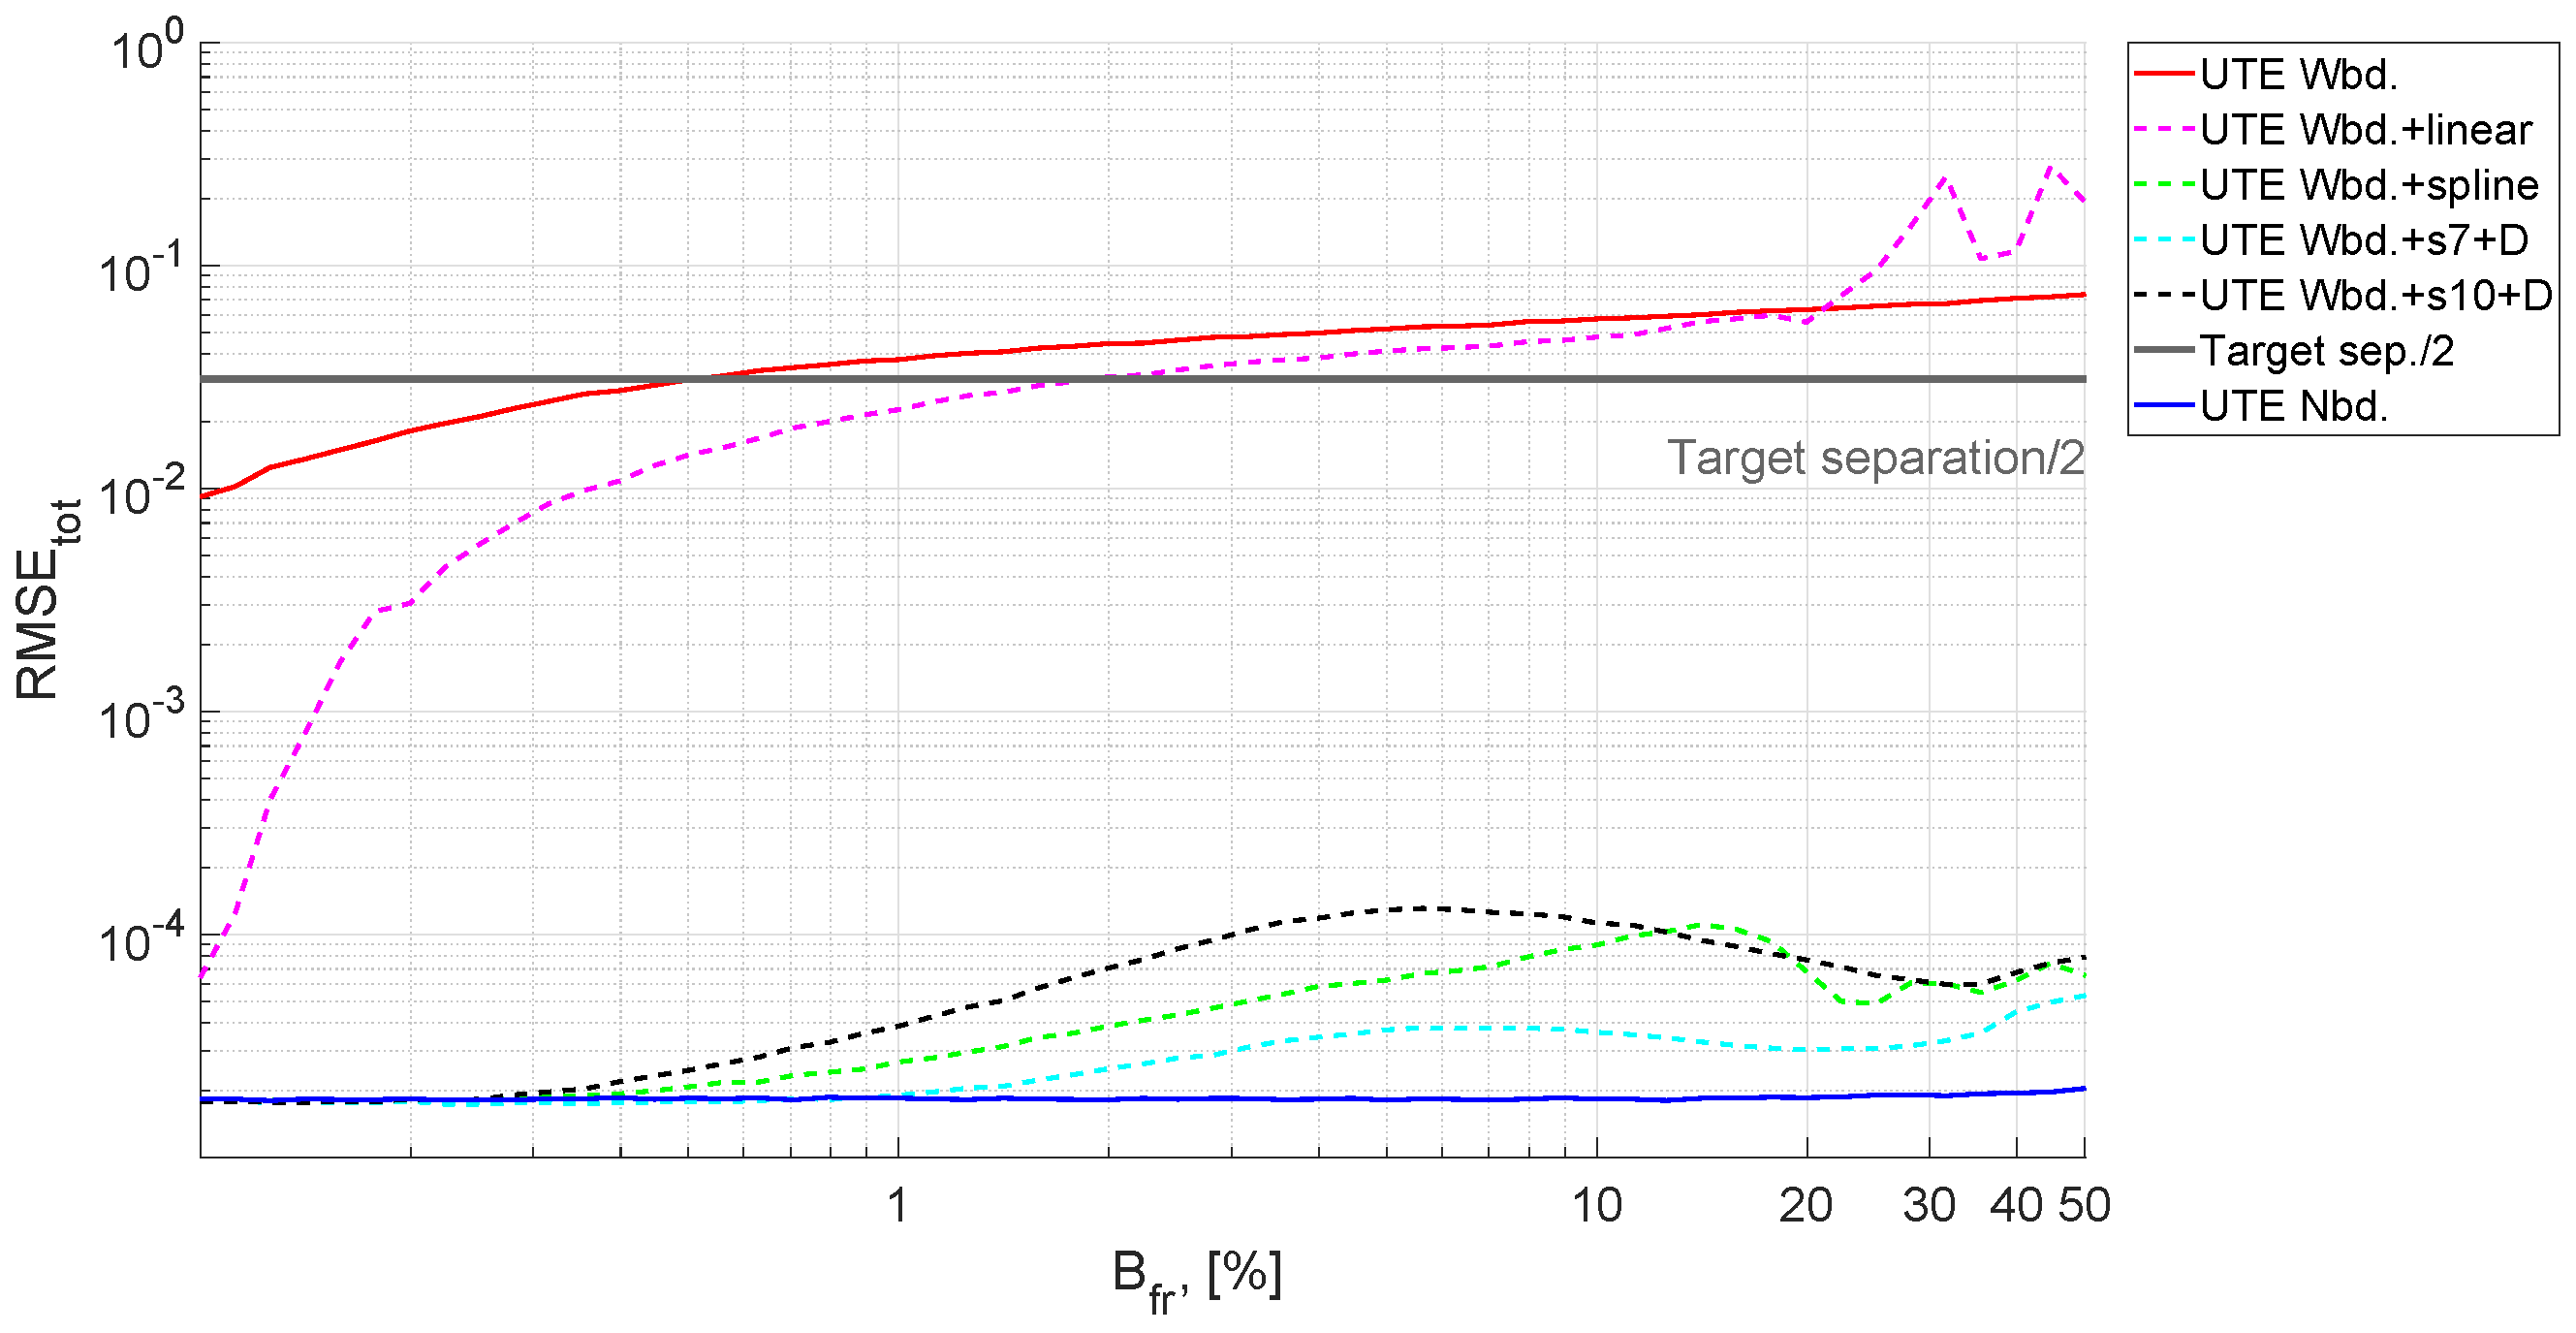
\includegraphics[scale=0.27]{FRAC_ed_final}
	}
	\caption{Среднеквадратическая ошибка оценивания в широкополосной системе.}
	\label{fig:ch2/sec1:frac}
\end{figure}

Например, на рисунке~\ref{fig:ch2/sec1:frac} изображена среднеквадратическая ошибка оценивания параметров канала связи (направлений прихода сигналов, относительной скорости, расстояния) в зависимости от относительной полосы частот системы.

На графике~\ref{fig:ch2/sec1:frac} изображены следующие кривые:
\begin{description}
	\item[<<UTE Nbd.>>] - <<Unitary Tensor Esprit>> алгоритм \cite{Haardt08}, применённый к узкополосной модели (данные сгенерированы при предположении $\sfr\approx\cfr$);
	\item[<<Target.sep./2>>] - половина минимального расстояния между отражателями в пространстве параметров;
	\item[<<UTE Wbd. + ... >>] -  <<Unitary Tensor Esprit>> алгоритм \cite{Haardt08}, применённый к широкополосной модели;
	\item[<<UTE Wbd. + linear >>] - использование линейной интерполяции для предварительной обработки принятых данных;
	\item[<<UTE Wbd. + spline >>] - использование интерполяции кубическими сплайнами для предварительной обработки принятых данных;
	\item[<<UTE Wbd. + s7/10 + D >>] - использование интерполяции сплайнами высокого порядка (7 и 10) для предварительной обработки принятых данных.
\end{description}

Результаты компьютерного моделирования показывают, что использование предварительной обработки с помощью интерполирования позволяет восстановить эффективность узкополосного алгоритма оценивания (UTE, \cite{Haardt08}). Эффективность пред-обработки зависит от величины относительной полосы частот рассматриваемой системы.

\let\pai\gpai

\section{Оценивание параметров каналов связи с отражателями в ближнем геометрическом поле}\label{ch:ch2/sec2}

Алгоритм TeNFiL и анализ его эффективности (диссертация Евгения), граница Крамера-Рао (диссертация Лианы), доработки.

\section{Анализ потенциальных характеристик оценивания параметров каналов связи при наличии негауссовских аддитивных помех}\label{ch:ch2/sec3}

\begin{comment}
Результаты данного раздела доклада были опубликованы в \cite{vakbib1}.

Планомерно растущие вычислительные способности программно-аппаратных комплексов обработки цифровых сигналов позволяют рассматривать всё более сложные модели данных и распределения аддитивных помех. Усложнение моделей задач, помимо повышения требований к вычислительным ресурсам, также несёт в себе потенциал для улучшения качественных показателей систем использующих цифровую обработку сигналов.

Задача оценивания направлений прихода заданного числа сигналов имеет множество приложений в области радиолокации и коммуникаций, а также, ввиду абстрактности и общеприменимости постановки, в сейсмологии, акустике, ультразвуковых измерениях. 

Задача имеет богатую историю в отечественной \cite{TrifShin1986, ManGel2015} и зарубежной \cite{Capon1969} литературе и продолжает оставаться актуальной. Аналитическое решение задачи отсутствует в литературе, поэтому распространение получили эвристические и численные методы решения. Среди первых стоит выделить класс методов подпространства сигналов \cite{Schmidt1986, Roy1989}, использующих спектральные разложения оценок пространственных ковариационных матриц. Для поиска оптимального решения зачастую применяются численные методы, такие как алгоритм IQML \cite{Bresler1985, Bresler1986}, итеративно максимизирующий функцию правдоподобия выборки, а также алгоритмы-производные от алгоритма EM, такие как MODE \cite{Stoica1990}. С точки зрения негауссовских аддитивных помех в литературе рассмотрен случай импульсного аддитивного шума, заданного смесью двух Гауссовских распределений с разными ковариациями \cite{Kozick2000, Kozick2000b}. Другой класс численных методов итеративно ищет оценку подпространства сигналов \cite{Ziskind1988, Bazzi2018}.

Для оценки эффективности этих алгоритмов, ввиду отсутствия других объективных критериев используется граница Крамера-Рао \cite{Cramer1993, KayS.1993}. Для случая аддитивного Гауссового шума выражение границы можно найти в \cite{Stoica1988, Stoica1989a, Stoica1989, Stoica1990a}, для случая импульсного шума выраженного смесью двух Гауссовых компонент с разными мощностями в \cite{Kozick2000, Kozick2000b, Kalyani2012}. Однако аналитический вывод границы Крамера-Рао в общем случае слишком сложен, и для произвольной смеси Гауссовых компонент отсутствует в литературе.

Целью работы в данном разделе являлся сравнительный анализ потенциальных характеристик оценивания параметров канала связи в виде направлений прихода сигналов массивом антенн в условиях различных моделей аддитивной помехи.

Для сравнения потенциальных характеристик используется нижняя граница Крамера-Рао. Для её вычисления предлагается метод вычисления нижней границы Крамера-Рао для произвольных распределений аддитивной помехи, а также проводится моделирование и сравнительный анализ данной границы для различных моделей аддитивной помехи.

Приведённый в данном разделе метод вычисления границы Крамера-Рао в задаче оценивания направлений прихода сигналов для общего выражения распределения аддитивной помехи основывается на алгоритме Монте-Карло, который используется для оценки информационной матрицы Фишера аддитивной помехи. Данная матрица затем используется для вычисления границы Крамера-Рао для оцениваемых параметров. Метод является общеприменимым до тех пор пока имеется возможность генерации отсчётов помехи.


\section{Одиночное изображение}\label{sec:ch2/sec1}

\begin{figure}[ht]
  \centerfloat{
    \includegraphics[scale=0.27]{latex}
  }
  \caption{TeX.}\label{fig:latex}
\end{figure}

Для выравнивания изображения по-центру используется команда \verb+\centerfloat+, которая является во
многом улучшенной версией встроенной команды \verb+\centering+.

\section{Длинное название параграфа, в котором мы узнаём как сделать две картинки с~общим номером и названием}\label{sec:ch2/sect2}

А это две картинки под общим номером и названием:
\begin{figure}[ht]
  \begin{minipage}[b][][b]{0.49\linewidth}\centering
    \includegraphics[width=0.5\linewidth]{knuth1} \\ а)
  \end{minipage}
  \hfill
  \begin{minipage}[b][][b]{0.49\linewidth}\centering
    \includegraphics[width=0.5\linewidth]{knuth2} \\ б)
  \end{minipage}
  \caption{Очень длинная подпись к изображению,
      на котором представлены две фотографии Дональда Кнута}
  \label{fig:knuth}
\end{figure}

Те~же~две картинки под~общим номером и~названием,
но с автоматизированной нумерацией подрисунков:
\begin{figure}[ht]
    \centerfloat{
        \hfill
        \subcaptionbox[List-of-Figures entry]{Первый подрисунок\label{fig:knuth_2-1}}{%
            \includegraphics[width=0.25\linewidth]{knuth1}}
        \hfill
        \subcaptionbox{\label{fig:knuth_2-2}}{%
            \includegraphics[width=0.25\linewidth]{knuth2}}
        \hfill
        \subcaptionbox{Третий подрисунок, подпись к которому
        не~помещается на~одной строке}{%
            \includegraphics[width=0.3\linewidth]{example-image-c}}
        \hfill
    }
    \legend{Подрисуночный текст, описывающий обозначения, например. Согласно
    ГОСТ 2.105, пункт 4.3.1, располагается перед наименованием рисунка.}
    \caption[Этот текст попадает в названия рисунков в списке рисунков]{Очень
    длинная подпись к второму изображению, на~котором представлены две
    фотографии Дональда Кнута}\label{fig:knuth_2}
\end{figure}

На рисунке~\ref{fig:knuth_2-1} показан Дональд Кнут без головного убора.
На рисунке~\ref{fig:knuth_2}\subcaptionref*{fig:knuth_2-2}
показан Дональд Кнут в головном уборе.

Возможно вставлять векторные картинки, рассчитываемые \LaTeX\ <<на~лету>>
с~их~предварительной компиляцией. Надписи в таких рисунках будут выполнены
тем же~шрифтом, который указан для документа в целом.
На~рисунке~\ref{fig:tikz_example} на~странице~\pageref{fig:tikz_example}
представлен пример схемы, рассчитываемой пакетом \verb|tikz| <<на~лету>>.
Для ускорения компиляции, подобные рисунки могут быть <<кешированы>>, что
определяется настройками в~\verb|common/setup.tex|.
Причём имя предкомпилированного
файла и~папка расположения таких файлов могут быть отдельно заданы,
что удобно, если не~для подготовки диссертации,
то~для подготовки научных публикаций.
\begin{figure}[ht]
    \centerfloat{
        \ifdefmacro{\tikzsetnextfilename}{\tikzsetnextfilename{tikz_example_compiled}}{}% присваиваемое предкомпилированному pdf имя файла (не обязательно)
        \input{Dissertation/images/tikz_scheme.tikz}

    }
    \legend{}
    \caption[Пример \texttt{tikz} схемы]{Пример рисунка, рассчитываемого
        \texttt{tikz}, который может быть предкомпилирован}\label{fig:tikz_example}
\end{figure}

Множество программ имеют либо встроенную возможность экспортировать векторную
графику кодом \verb|tikz|, либо соответствующий пакет расширения.
Например, в GeoGebra есть встроенный экспорт,
для Inkscape есть пакет svg2tikz,
для Python есть пакет matplotlib2tikz,
для R есть пакет tikzdevice.

\section{Пример вёрстки списков}\label{sec:ch2/sec3}

\noindent Нумерованный список:
\begin{enumerate}
  \item Первый пункт.
  \item Второй пункт.
  \item Третий пункт.
\end{enumerate}

\noindent Маркированный список:
\begin{itemize}
  \item Первый пункт.
  \item Второй пункт.
  \item Третий пункт.
\end{itemize}

\noindent Вложенные списки:
\begin{itemize}
  \item Имеется маркированный список.
  \begin{enumerate}
    \item В нём лежит нумерованный список,
    \item в котором
    \begin{itemize}
      \item лежит ещё один маркированный список.
    \end{itemize}
  \end{enumerate}
\end{itemize}

\noindent Нумерованные вложенные списки:
\begin{enumerate}
  \item Первый пункт.
  \item Второй пункт.
  \item Вообще, по ГОСТ 2.105 первый уровень нумерации
  (при необходимости ссылки в тексте документа на одно из перечислений)
  идёт буквами русского или латинского алфавитов,
  а второй "--- цифрами со~скобками.
  Здесь отходим от ГОСТ.
    \begin{enumerate}
      \item в нём лежит нумерованный список,
      \item в котором
        \begin{enumerate}
          \item ещё один нумерованный список,
          \item третий уровень нумерации не нормирован ГОСТ 2.105;
          \item обращаем внимание на строчность букв,
          \item в этом списке
          \begin{itemize}
            \item лежит ещё один маркированный список.
          \end{itemize}
        \end{enumerate}

    \end{enumerate}

  \item Четвёртый пункт.
\end{enumerate}

\section{Традиции русского набора}

Много полезных советов приведено в материале
<<\href{http://www.dropbox.com/s/x4hajy4pkw3wdql/wholesome-typesetting.pdf?dl=1\&pv=1}{Краткий курс благородного набора}>> (автор А.\:В.~Костырка).
Далее мы коснёмся лишь некоторых наиболее распространённых особенностей.

\subsection{Пробелы}

В~русском наборе принято:
\begin{itemize}
    \item единицы измерения, знак процента отделять пробелами от~числа:
        10~кВт, 15~\% (согласно ГОСТ 8.417, раздел 8);
    \item \(\tg 20\text{\textdegree}\), но: 20~{\textdegree}C
        (согласно ГОСТ 8.417, раздел 8);
    \item знак номера, параграфа отделять от~числа: №~5, \S~8;
    \item стандартные сокращения: т.\:е., и~т.\:д., и~т.\:п.;
    \item неразрывные пробелы в~предложениях.
\end{itemize}

\subsection{Математические знаки и символы}

Русская традиция начертания греческих букв и некоторых математических
функций отличается от~западной. Это исправляется серией
\verb|\renewcommand|.
\begin{itemize}
%Все \original... команды заранее, ради этого примера, определены в Dissertation\userstyles.tex
    \item[До:] \( \originalepsilon \originalge \originalphi\),
    \(\originalphi \originalleq \originalepsilon\),
    \(\originalkappa \in \originalemptyset\),
    \(\originaltan\),
    \(\originalcot\),
    \(\originalcsc\).
    \item[После:] \( \epsilon \ge \phi\),
    \(\phi \leq \epsilon\),
    \(\kappa \in \emptyset\),
    \(\tan\),
    \(\cot\),
    \(\csc\).
\end{itemize}

Кроме того, принято набирать греческие буквы вертикальными, что
решается подключением пакета \verb|upgreek| (см. закомментированный
блок в~\verb|userpackages.tex|) и~аналогичным переопределением в
преамбуле (см.~закомментированный блок в~\verb|userstyles.tex|). В
этом шаблоне такие переопределения уже включены.

Знаки математических операций принято переносить. Пример переноса
в~формуле~\eqref{eq:equation3}.

\subsection{Кавычки}
В английском языке приняты одинарные и двойные кавычки в~виде ‘...’ и~“...”.
В России приняты французские («...») и~немецкие („...“) кавычки (они называются
«ёлочки» и~«лапки», соответственно). ,,Лапки`` обычно используются внутри
<<ёлочек>>, например, <<... наш гордый ,,Варяг``...>>.

Французкие левые и правые кавычки набираются
как лигатуры \verb|<<| и~\verb|>>|, а~немецкие левые
и правые кавычки набираются как лигатуры \verb|,,| и~\verb|‘‘| (\verb|``|).

Вместо лигатур или команд с~активным символом "\ можно использовать команды
\verb|\glqq| и \verb|\grqq| для набора немецких кавычек и команды \verb|\flqq|
и~\verb|\frqq| для набора французских кавычек. Они определены в пакете
\verb|babel|.

\subsection{Тире}
%  babel+pdflatex по умолчанию, в polyglossia надо включать опцией (и перекомпилировать с удалением временных файлов)
Команда \verb|"---| используется для печати тире в тексте. Оно несколько короче
английского длинного тире. Кроме того, команда задаёт небольшую жёсткую отбивку
от слова, стоящего перед тире. При этом, само тире не~отрывается от~слова.
После тире следует такая же отбивка от текста, как и~перед тире. При наборе
текста между словом и командой, за которым она следует, должен стоять пробел.

В составных словах, таких, как <<Закон Менделеева"--~Клапейрона>>, для печати
тире надо использовать команду \verb|"--~|. Она ставит более короткое,
по~сравнению с~английским, тире и позволяет делать переносы во втором слове.
При~наборе текста команда \verb|"--~| не отделяется пробелом от слова,
за~которым она следует (\verb|Менделеева"--~|). Следующее за командой слово
может быть  отделено от~неё пробелом или перенесено на другую строку.

Если прямая речь начинается с~абзаца, то перед началом её печатается тире
командой \verb|"--*|. Она печатает русское тире и жёсткую отбивку нужной
величины перед текстом.

\subsection{Дефисы и переносы слов}
%  babel+pdflatex по умолчанию, в polyglossia надо включать опцией (и перекомпилировать с удалением временных файлов)
Для печати дефиса в~составных словах введены две команды. Команда~\verb|"~|
печатает дефис и~запрещает делать переносы в~самих словах, а~команда \verb|"=|
печатает дефис, оставляя \TeX ’у право делать переносы в~самих словах.

В отличие от команды \verb|\-|, команда \verb|"-| задаёт место в~слове, где
можно делать перенос, не~запрещая переносы и~в~других местах слова.

Команда \verb|""| задаёт место в~слове, где можно делать перенос, причём дефис
при~переносе в~этом месте не~ставится.

Команда \verb|",| вставляет небольшой пробел после инициалов с~правом переноса
в~фамилии.

\section{Текст из панграмм и формул}

\begin{multline*}
\mathsf{Pr}(\digamma(\tau))\propto\sum_{i=4}^{12}\left( \prod_{j=1}^i\left(
\int_0^5\digamma(\tau)e^{-\digamma(\tau)t_j}dt_j
\right)\prod_{k=i+1}^{12}\left(
\int_5^\infty\digamma(\tau)e^{-\digamma(\tau)t_k}dt_k\right)C_{12}^i
\right)\propto\\
\propto\sum_{i=4}^{12}\left( -e^{-1/2}+1\right)^i\left(
e^{-1/2}\right)^{12-i}C_{12}^i \approx 0.7605,\quad
\forall\tau\neq\overline{\tau}
\end{multline*}

%Большая фигурная скобка только справа
\[\left. %ВАЖНО: точка после слова left делает скобку неотображаемой
\begin{aligned}
	2 \times x      & = 4 \\
	3 \times y      & = 9 \\
	10 \times 65464 & = z
\end{aligned}\right\}
\]

\end{comment}     % Глава 2
% \include{Dissertation/part3}     % Глава 3

\clearpage
\chapter{Заключение}
Основные результаты работы заключаются в следующем:
%% Согласно ГОСТ Р 7.0.11-2011:
%% 5.3.3 В заключении диссертации излагают итоги выполненного исследования, рекомендации, перспективы дальнейшей разработки темы.
%% 9.2.3 В заключении автореферата диссертации излагают итоги данного исследования, рекомендации и перспективы дальнейшей разработки темы.

\begin{itemize}
\item предложен метод предварительной обработки многомерных сигналов в широкополосных системах, позволяющий применять алгоритмы оценивания параметров каналов связи, разработанные для узкополосных систем. Предложенный метод предварительной обработки многомерных сигналов в широкополосных системах существенно повышает точность алгоритмов оценки параметров каналов связи, разработанных для узкополосных систем. Улучшение точности оценивания увеличивается при увеличении относительной полосы частот рассматриваемой широкополосной системы. Например, показана эффективность данного метода в широкополосных системах с относительной полосой частот, превышающей 10\%; 
\item разработан новый алгоритм оценивания параметров канала связи с отражателями в ближнем геометрическом поле с использованием сферической модели фронта волны. С помощью компьютерного моделирования показано, что разработанный алгоритм оценивания параметров канала связи с отражателями в ближнем геометрическом поле более эффективен чем существующие алгоритмы;
\item впервые исследована граница Крамера-Рао для задач оценки параметров каналов связи с негауссовым распределением аддитивной помехи, заданным смесью нормальных распределений с ненулевыми средними значениями компонент. Показано, что использование более сложных моделей аддитивных помех, в частности с негауссовским распределением аддитивной помехи, выраженным смесью нормальных распределений, потенциально позволяет увеличить точность работы алгоритмов оценивания параметров каналов связи;
\item разработана программная реализация предложенных алгоритмов, а также компьютерные модели, имитирующие работу инфокоммуникационных систем с предложенными алгоритмами и оценивающие эффективность их работы.
\end{itemize}

\begin{comment}
Результаты математического моделирования показали практическую применимость метода вычисления нижней границы Крамера-Рао. Используя данный метод граница может быть вычислена при произвольном распределении аддитивной помехи. Результаты моделирования также показали, что граница Крамера-Рао ниже для сложных распределений аддитивных помех. Следовательно, алгоритмы на основе сложных моделей аддитивных помех содержат потенциал к улучшению качества оценивания искомых параметров, и, как следствие, к улучшению качественных показателей функционирования систем радиолокации и телекоммуникаций.
\end{comment}

\clearpage
\addcontentsline{toc}{chapter}{Публикации автора по теме диссертации}
\ifdefmacro{\microtypesetup}{\microtypesetup{protrusion=false}}{} % не рекомендуется применять пакет микротипографики к автоматически генерируемому списку литературы
\urlstyle{rm}                               % ссылки URL обычным шрифтом
\ifnumequal{\value{bibliosel}}{0}{% Встроенная реализация с загрузкой файла через движок bibtex8
  \renewcommand{\bibname}{\large \bibtitleauthor}
  \nocite{*}
  \insertbiblioauthor           % Подключаем Bib-базы
  %\insertbiblioexternal   % !!! bibtex не умеет работать с несколькими библиографиями !!!
}{% Реализация пакетом biblatex через движок biber
  % Цитирования.
  %  * Порядок перечисления определяет порядок в библиографии (только внутри подраздела, если `\insertbiblioauthorgrouped`).
  %  * Если не соблюдать порядок "как для \printbibliography", нумерация в `\insertbiblioauthor` будет кривой.
  %  * Если цитировать каждый источник отдельной командой --- найти некоторые ошибки будет проще.
  %
  %% authorvak
  % \nocite{*}
  % \nocite{vakbib1}%
  % \nocite{vakbib2}%
  %
  %% authorscopus
  \nocite{Zhang2017}%
  % \nocite{Podkurkov2017}%
  %
  %% authorconf
  % \nocite{Zhang2016}%
  % \nocite{ptitt18}%
  % \nocite{Podkurkov2018}%
  %% authorwos
  % \nocite{Podkurkov2019}%
  %% authorother
  % \nocite{otherbib1}%
  %
  \ifnumgreater{\value{usefootcite}}{0}{
    \begin{refcontext}[labelprefix={}]
      \ifnum \value{bibgrouped}>0
        \insertbiblioauthorgrouped    % Вывод всех работ автора, сгруппированных по источникам
      \else
        \insertbiblioauthor      % Вывод всех работ автора
      \fi
    \end{refcontext}
  }{
  \ifnum \value{citeexternal}>0
    \begin{refcontext}[labelprefix=A]
      \ifnum \value{bibgrouped}>0
        \insertbiblioauthorgrouped    % Вывод всех работ автора, сгруппированных по источникам
      \else
        \insertbiblioauthor      % Вывод всех работ автора
      \fi
    \end{refcontext}
  \else
    \ifnum \value{bibgrouped}>0
      \insertbiblioauthorgrouped    % Вывод всех работ автора, сгруппированных по источникам
    \else
      \insertbiblioauthor      % Вывод всех работ автора
    \fi
  \fi
  %  \insertbiblioauthorimportant  % Вывод наиболее значимых работ автора (определяется в файле characteristic во второй section)
  \begin{refcontext}[labelprefix={}]    \insertbiblioexternal            % Вывод списка литературы, на которую ссылались в тексте автореферата
  \end{refcontext}
  }
}
\ifdefmacro{\microtypesetup}{\microtypesetup{protrusion=true}}{}
\urlstyle{tt}                               % возвращаем установки шрифта ссылок URL
      % Содержание автореферата


\end{document}
